\chapter{I Had \$78\ldots\ Now I'm Worth \$100 Million}

This lecture begins in spectacle and then spends the rest of its time undoing the spectacle. We start with the plane, with money, with access, and with the blunt question of how one gets there. But the interview does not stay at the level of image. It steadily translates image into arithmetic: a tail number becomes a memory of \$78, a jet becomes a recurring operating burden, a healthcare business becomes a funnel, sleep becomes a hard input into cognition, and scale becomes a question of leverage, bankability, and disciplined attention. Read in that way, the lecture is not a piece of motivational theater. It is a sequence of thresholds.

\section{Jet, Tail Number, and the Arithmetic of Proof}

The opening is structured as a challenge. We are shown the private jet first because that is what the audience wants to see. Then, almost immediately, the lecture asks us to decide whether the thing is real. The answer is numerical before it is philosophical:
\begin{align}
4 &\mapsto \text{April}, &
78 &\mapsto \$78, \\
C_{\text{jet}} &> \$5\,\text{million}, &
O_{\text{jet,yr}} &\approx \$2\,\text{million/year}.
\end{align}
The first line is symbolic. The second is economic. The lecture wants the audience to feel the shift from ornament to burden.

We should be a little careful with the first line. The mapping
\[
4 \mapsto \text{April}, \qquad 78 \mapsto \$78
\]
is not bookkeeping. It is compressed autobiography. The tail number matters because it is a private mnemonic turned public sign: birth month on one side, rock bottom on the other.

The second line is the more serious move. A private jet is not treated as a purchase alone, but as a continuing obligation. That point is sharpened by the speaker’s own example: even if somebody gave you the plane, you would still have to carry the operating cost. In a compact form,
\begin{align}
C_{\text{jet}} &\to 0 \quad \text{(gift case)}, \\
O_{\text{jet,yr}} &\not\to 0.
\end{align}
So the relevant threshold is not ownership in the abstract; it is recurring cash flow. The lecture later states the practical affordability rule more explicitly:
\begin{equation}
I_{\text{disp}} \gtrsim O_{\text{jet,yr}} \approx \$2\,\text{million/year},
\end{equation}
and then sharpens that into a rule of thumb:
\begin{equation}
I_{\text{disp}} \in [\$2,\$3]\,\text{million/year}.
\end{equation}
We should not pretend this is an audited aviation model. It is a speaker-reported threshold. But it is the correct kind of threshold for the lecture, because it transforms the plane from spectacle into proof.

There is a short travel-log interlude in which the host narrates being flown from Miami to Tampa. That interlude is not wasted time. It shows that the jet is already doing work in the argument. It changes the geography of the conversation. It makes the interview possible on these terms. Access has entered before the formal discussion has even started.

\section{From \$78 to Commitment}

Once the tail number is decoded, the lecture asks its first operative question. The symbol now has to become a method. What does one actually do when one is down to \$78?

\subsection{Question \& Answer}

\paragraph{Question.} What is the first actionable step when you are down to \$78 and do not yet know how to start?

\paragraph{Answer.} The speaker’s answer is not a tactic, a platform, or a product category. It is commitment. More precisely, it is the refusal to let the goal remain optional.

This matters because the lecture is careful not to offer a fake causality. It does not say that commitment mechanically produces cash. It says something narrower and more defensible: without commitment, no later mechanism survives long enough to matter. A good idea without commitment collapses at the first serious resistance.

We can state the logic schematically. When capital is near zero, the first threshold is not financial but positional. The entrepreneur has to stop treating the project as one possible path among many and start treating it as the dominant object around which the rest of life is arranged. That is why the answer is expressed in absolute language: nothing was more important, not comfort, not convenience, not sleep, not the ordinary wish to back away.

The lecture immediately follows this with a payoff, and that payoff should remain close to the answer. The speaker is asked whether the sacrifice was worth it, and he replies in two currencies at once: yes, because of the money, and yes, because of the quality of life. He then gives the first sign that success is not merely symbolic. He mentions Medell\'{\i}n, an office there, a house there, and a workforce of roughly \(350\) employees there. So the first answer does not end in rhetoric. It ends in operating range.

\section{A Niche Healthcare Machine, Not a Glamour Startup}

Only after commitment has been fixed does the lecture show us the machine to which commitment was applied. This order is important. The interview does not begin with an abstract lecture on industry selection. It first asks whether one is serious at all, and only then lets us examine the field.

The field is Blackstone Medical Services, described as the largest provider of medical sleep testing in the United States. The scale markers are concrete:
\begin{align}
t_{\text{start}} &= 2012, \\
N_{\text{emp}} &> 650, \\
N_{\text{pat}} &> 10^6.
\end{align}
We are also told that the early business handled only a few hundred patients per month, and that by May of the present year cumulative tested-patient volume had exceeded one million. The chapter should preserve that contrast because it is the lecture’s simplest scale story: a kitchen start, a tiny monthly flow, and then an eventual million-patient milestone.

The host calls the business niche and even a little unsexy. That is exactly the point. The lecture is pushing against the fantasy that serious wealth must begin in a glamorous technology category. Here the business is institutional, repetitive, medically narrow, and operationally heavy. It wins not by dazzling the culture but by solving a real problem inside a system.

The speaker then gives the lecture’s emotional justification for staying in that system. He says, in effect, that passion is not a substitute for execution, but it is what keeps execution alive through the headaches and the delays. The biographical support for that claim is also specific: his parents died of cancer when he was young, so healthcare was not a random market. It was already charged with personal attention. That is why the lecture moves so naturally from niche into passion and then from passion into performance.

\section{Sleep as an Operating Constraint}

The subject now bends back on the operator. Because the business lives in sleep medicine, the host asks what sleep has to do with success. The answer is crisp: sleep is an input into business performance.

The speaker’s personal threshold is given directly:
\begin{align}
h_{\text{sleep}} &\in [6,7]\ \text{hours/night}, \\
h_{\text{sleep}} < h_{\min} &\Rightarrow \text{drag, weaker focus, poorer meeting attention}.
\end{align}
This is not a universal physiological theorem. It is a local operating law, and the lecture treats it as such. But the local law matters because the business world described in the interview is one of \(12\)- to \(14\)-hour days, long meetings, and sustained concentration. Once we grant that, degraded attention becomes an economic variable.

\subsection{Question \& Answer}

\paragraph{Question.} Does sleep actually matter for entrepreneurial performance, or is sleep deprivation part of the myth of hustle?

\paragraph{Answer.} In the lecture, sleep matters because entrepreneurship is treated as cognitive endurance. If the brain is underfed or underrested, the operator cannot hold the day together. So the slogan that sleep is for weak people is rejected not on moral grounds, but on functional grounds.

This is a good example of the lecture’s rhythm. It does not stay in abstraction. It moves from a business niche to a physiological claim and then immediately uses that claim as a bridge back to the actual start of the company.

\section{Kitchen Start and the Market Funnel}

Now we descend from threshold language into the small machinery of the beginning. The speaker describes pajamas, a white desk, an Apple computer, a divorce, two young children, and the experience of starting over. The scene could easily be romanticized. The lecture resists that by turning the scene into process.

The first process claim concerns the structure of the market. The United States is described as an insured environment:
\begin{equation}
r_{\text{insured}} \approx 0.97.
\end{equation}
That claim motivates the first side of the funnel. If most patients are entering care through insurance, then insurer contracts are not optional. The second side is doctor-side business development. Each morning begins with email outreach to insurance companies. The day continues with calls on physicians. Only after both sides are in motion does patient volume begin to accumulate.

A cautious reconstruction is therefore
\begin{equation}
F_{\text{patients}} = F(C_{\text{ins}},D_{\text{doc}}),
\end{equation}
where \(C_{\text{ins}}\) denotes insurer contracting and \(D_{\text{doc}}\) denotes doctor acquisition or doctor-side referral relationships. This formula is schematic only. The interview provides no functional form and no conversion rates. But the schematic is valuable because it captures the lecture’s real sequence: insurer access, doctor access, patient flow.

The first office belongs inside the same chain:
\begin{equation}
R_{\text{office}} = \$500/\text{month}, \qquad A_{\text{office}} \approx 500\ \text{ft}^2.
\end{equation}
That office is not important because it is large. It is important because it is measurable. Once again the lecture is taking a story and crystallizing it into a number.

\begin{figure}
\centering
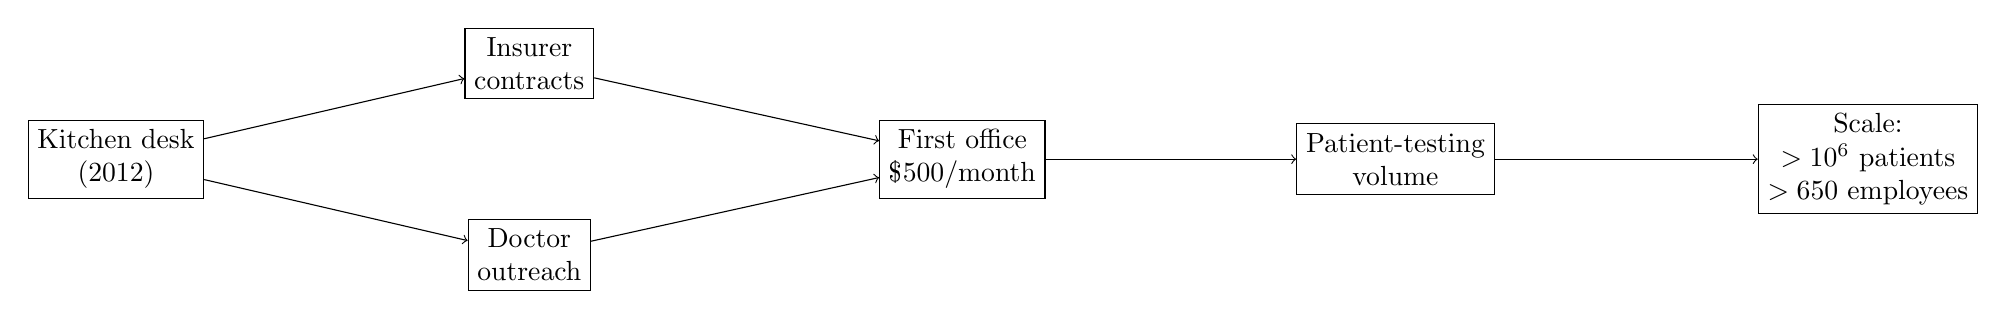
\begin{tikzpicture}[x=2.5cm,y=1.35cm]
\node[draw, rectangle, align=center] (k) at (0,0) {Kitchen desk\\(2012)};
\node[draw, rectangle, align=center] (i) at (2.1,0.9) {Insurer\\contracts};
\node[draw, rectangle, align=center] (d) at (2.1,-0.9) {Doctor\\outreach};
\node[draw, rectangle, align=center] (o) at (4.3,0) {First office\\\$500/month};
\node[draw, rectangle, align=center] (p) at (6.5,0) {Patient-testing\\volume};
\node[draw, rectangle, align=center] (s) at (8.9,0) {Scale:\\\(>10^6\) patients\\\(>650\) employees};
\draw[->] (k) -- (i);
\draw[->] (k) -- (d);
\draw[->] (i) -- (o);
\draw[->] (d) -- (o);
\draw[->] (o) -- (p);
\draw[->] (p) -- (s);
\end{tikzpicture}
\caption{A transcript-derived reconstruction of the startup funnel described in the interview.}
\end{figure}

The figure should be read as a cleaned schematic of the spoken sequence, not as a hidden board diagram. Its purpose is modest: to preserve the lecture’s order and to prevent the kitchen story from dissolving into generic bootstrap mythology.

\section{Service, Team, and the Founder at Scale}

The lecture now asks what actually created the business outcome. The answer is given in layers. First, there are many products in the market. So product alone is not the source of leadership. The speaker insists that what separates the firm is everything that goes with the product, above all the service layer. If we want a compact notation for that thought, we may write
\begin{equation}
Q_{\text{offer}} = Q_{\text{product}} + Q_{\text{service}},
\end{equation}
but we should remember that this is a careful compression of the spoken argument, not the speaker’s literal algebra.

Second, the lecture introduces a recent wealth claim:
\begin{equation}
\Delta W_{3\text{--}4\text{ yr}} \approx \$85\,\text{million}.
\end{equation}
The host immediately asks what moved the needle. The answer is not more founder heroics. It is investment in the right team. Indeed, the speaker says that there was a period when his staff earned more than he did, and that he was willing to accept that because the business needed scale more than it needed the founder’s ego to be protected.

This gives us the central leverage claim of the chapter:
\begin{equation}
N_{\text{emp}} \gg 1 \quad \Rightarrow \quad Y_{\text{firm}} \not\approx Y_{\text{founder-alone}}.
\end{equation}
That formula must be read carefully. The speaker also says, with great emphasis, that the founder remains the most important person in the business. There is no contradiction. Importance and throughput are not the same variable. The founder may remain decisive while the firm’s output becomes organizational rather than personal.

\subsection{Question \& Answer}

\paragraph{Question.} What actually moves the needle once the company is too large for founder labor alone?

\paragraph{Answer.} The lecture’s answer is team leverage. One still needs the founder’s will, vision, and self-belief. But a \(650\)-person company cannot be run as a one-man performance. Scale enters precisely when the founder pays for capability in others and allows the system to become larger than his own hands.

The lecture then turns briefly inward again. The speaker calls himself the most important person in the business, says that one must bet on oneself, and describes dark periods in which quitting was never an option. These are not decorative remarks. They explain why the earlier leverage claim does not become a bureaucratic claim. The system scales, but the organizing center remains intensely personal.

\section{Bankability, Mentors, and the Discipline of Thinking}

Once the question of leverage has been answered, the interview becomes more infrastructural. The speaker is asked which people matter most in building the business. The answer arrives as a triad: accountant, operations lead, CTO. Their order matters.

Accounting comes first because the lecture now introduces bankability. Clean books and trustworthy numbers are not clerical niceties. They are the precondition for credit access, for sale-readiness, and for the ability to be taken seriously by institutions:
\begin{equation}
\text{clean books} \Rightarrow B_{\text{bankable}} \Rightarrow \text{credit access and sale readiness}.
\end{equation}
The operations lead is the person in the weeds. The CTO is the person asked to think in a \(3\)-to-\(5\)-year arc. What was earlier presented as hustle is now presented as institution-building.

There is a brief host interlude here about bookkeeping software. The advertisement is incidental. The mathematical point is not incidental. A real business is one whose numbers can be trusted.

From bankability the lecture turns to mentors, and then from mentors to thought-style. The speaker says that he remains a student and that the moment one believes one knows everything, one is finished. This matters because the lecture is no longer only about what to do. It is about how to stay corrigible while doing it.

The mentor anecdote about bagels and coffee is the cleanest example. A very wealthy man refuses to pay an inflated incidental charge on a private flight, not because he lacks the money but because the line item does not correspond to what the thing intrinsically costs. The lesson is that wealth does not suspend arithmetic. On the contrary, arithmetic becomes more important because wealth makes overspending easy. This is the lecture’s version of shrewdness.

The same style of thinking appears in negotiation. The rule is simple: do not give the first number. If \(a_1\) is the first anchor, then the lecture’s practical law is
\begin{equation}
\text{do not set } a_1 \text{ first.}
\end{equation}
The reason is equally simple. The first number reveals a range before the other side has exposed its own. The speaker does not wrap this in formal bargaining theory, but the operational logic is perfectly clear.

Now the lecture widens again into competition. The industry once had large incumbents. One major competitor was still active in 2018; around 2019 the speaker says his firm passed it in volume:
\begin{equation}
t_{\text{overtake}} \approx 2019.
\end{equation}
From that point on, the stated mechanism of persistence is consistency. Thousands of patients are moving through the system every day, and there is no room for an extended lapse. The phrase is almost mechanical: deliver over and over and over again.

The lecture closes this cluster with a threshold metaphor: water boils at \(212\), not \(211\). We should not literalize it. The point is that decisive edges may appear small in notation and enormous in outcome.

\subsection{Question \& Answer}

\paragraph{Question.} When does a private jet become a business tool rather than a fantasy image?

\paragraph{Answer.} It becomes a business tool only after the cash-flow threshold has already been crossed:
\begin{align}
I_{\text{disp}} &\in [\$2,\$3]\,\text{million/year}, \\
I_{\text{disp}} &\gtrsim O_{\text{jet,yr}}.
\end{align}
Once that happens, the jet changes category. It is no longer merely transport. It becomes an access machine. The speaker says directly that he networks with more billionaires after getting the plane, and that he can now call people and bring them into motion with him. The plane also changes family logistics, work range, and the density of high-value conversation. So the lecture ends where it began, but under a different description. The jet is no longer spectacle; it is downstream capital.

\section{Summary}

The interview begins by showing us a plane and then teaches us how to read it. The tail number becomes a symbolic memory of \$78. The jet becomes a recurring operating burden. Commitment becomes the first threshold. A niche healthcare business becomes an institutional machine. Sleep becomes a cognitive floor. A kitchen start unfolds into an insurer-and-doctor funnel. Product yields to service, service yields to team leverage, and team leverage yields to bankability and scale. Finally, the late doctrines of shrewdness, negotiation, consistency, and access gather the whole lecture back into one line of thought: visible wealth is never the starting point. It is the visible residue of thresholds that have already been crossed.